\documentclass{article}
\usepackage{fullpage}
\usepackage{graphicx}
\usepackage{../svn-multi}

\title{Proto Language Reference}
\author{By the authors of MIT Proto}
\date{Last Updated: \today}

\newcommand\todo[1]{\immediate\write16{TODO: #1}}
\newcommand\broken{{\em Not working!}}
\newcommand\nosecgen{{\em Not working in 2nd generation simulator!}}
\newcommand\bugs{{\em There are known bugs.}}
\newcommand\experimental{{\em Experimental: behavior may be flawed and 
    may be changed without warning.}}

\newcommand\violation{{\em Capable of violating the continuous
    space/time abstraction.}}

\newcommand\code[1]{\begin{quote}\var{#1}\end{quote}}
\newcommand\function[3]
{\begin{quote}{\tt #1}$\rightarrow$ \type{#2} \\ #3 \end{quote}}
\newcommand\type[1]{$#1$}
\newcommand\var[1]{{\tt #1}}

\begin{document}

\maketitle

This is a reference to all of the currently working functions in the
Proto language.  For a reference of commonly used simulator and
language commands, see the {\bf Proto Quick Start}.  For a tutorial on
the Proto language, see the document {\bf Thinking In Proto}.  For
installation instructions, see the {\bf README}.  For a user manual
for the simulator, see the {\bf Proto Simulator User Manual}.  For
information on how to extend the functionality of the simulator, see
the {\bf MIT Proto Developers Guide}.

This reference is intended as a ``dictionary'' to allow Proto
programmers to look up whether the function they are looking for
already exists, and how to use it.  This reference guide is organized
by groups of functionality.  It gives only minimal explanation of the
language, assuming that the programmer already understands the basics.

A note on implementation: some functions are implemented directly by
the Proto kernel, others are implemented by a mixture of kernel
functions and compiler pattern rewriting, and yet others are written
in Proto as part of the core library ({\tt lib/core/}).  This document
does not distinguish between these implementation decisions.

% standard LaTeX credits insert; should echo AUTHORS

\section{Credits for Proto}

The Proto language was created in partnership by Jonathan Bachrach and
Jacob Beal.  As they created the language, Jonathan created the first
implementation of MIT Proto, including the first compiler, kernel,
simulator, and embedded device implementations.  Since that time, Jake
and other contributors have built on the work begun by Jonathan.

MIT Proto also includes contributions from (alphabetically):
%
Aaron Adler, Geoffrey Bays, Anna Derbakova, Nelson Elhage, Takeshi
Fujiwara, Tony Grue, Joshua Horowitz, Tom Hsu, Kanak Kshetri, Prakash
Manghwani, Dustin Mitchell, Omar Mysore, Maciej Pacula, Hayes Raffle,
Dany Qumsiyeh, Omari Stephens, Mark Tobenkin, Ray Tomlinson, Kyle
Usbeck, Dan Vickery

The Protobo platform code in platforms/protobo/ also includes 
Topobo-related code from (alphabetically):
%
  Mike Fleder, Limor Fried, Josh Lifton, Laura Yip



\section{Notation}

Functions and special forms in this document are specified in a
pattern language closely related to the quasiquote metasyntax used in
LISPs.
\begin{itemize}
\item {\tt .name} means $name$ is a variable that matches only identifiers. 
\item {\tt ,name} means $name$ is a variable that matches any expression.
\item {\tt ,@name} means $name$ is a variable that matches a list of
  expressions, at least one expression long.
\item {\tt ...} indicates zero or more of the preceding pattern element.
\item {\tt ++} indicates one or more of the preceding pattern element.
\item {\tt var|\type{type}} means that $var$ must be of data type
  $type$.  If there is no type specified, it means the variable can be
  any type.
\end{itemize}

Throughout the document Proto functions and special forms are
expressed as: 
\function{pattern}{type}{description}
where \type{type} is the return type.

The names of functions are in all lower case; the names of special
forms are in all upper case.


\section{Evaluation}

Proto is a purely functional language.  Proto is written using
s-expressions in a manner very similar to Scheme.  Evaluating a Proto
expression produces a program: a dataflow graph that may be evaluated
against a space to produce an evolving field of values at every point
on the space.


\section{Data Types}

All Proto expressions produce fields that map every point in space to
a value.  The values produced are categorized into the type system
shown in Figure~\ref{f:types}.

\begin{figure}[hp]
\centering
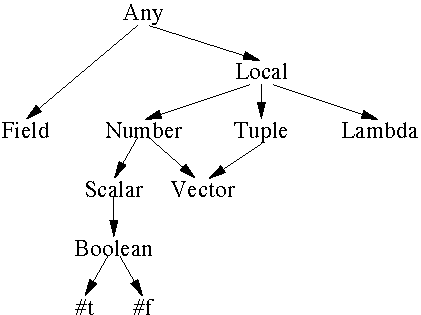
\includegraphics{figures/types.pdf}
\caption{Proto data types; arrows indicate subset relationships.}
\label{f:types}
\end{figure}

\begin{itemize}
\item {\bf Any} is the top type, encompassing all other types.
\item {\bf Field} is a function mapping a subset of the device's
  neighborhood to {\bf Local} values.
\item {\bf Local} is any non-{\bf Field} value: a {\bf Number}, 
  {\bf Tuple}, or {\bf Lambda}.
\item {\bf Lambda} is a function.
\item {\bf Tuple} is an ordered set of $k$ {\bf Local} values.
\item {\bf Scalar} is a floating point number (including the special
  values {\tt Inf}, {\tt -Inf}, and {\tt NaN}).
\item {\bf Vector} is a {\bf Tuple} of {\bf Scalar} values.
\item {\bf Number} is a {\bf Scalar} or {\bf Vector}.
\item {\bf Boolean} is a {\bf Scalar} interpreted as a logical value.
  True is any non-zero value, canonically {\bf \#t}, which is
  represented by 1; False, canonically {\bf \#f}, is represented by 0.
\end{itemize}

Throughout this document, types will be abbreviated by their first
letter, except for {\bf Lambda}, which will be abbreviated as
$\lambda$.  Tuples and vectors may be further specified by a subscript
indicating length (e.g. \type{T_3} is a tuple of 3 elements), and
tuples may also have their types specified as a parenthetical list
(e.g. \type{T(T_2,S)} is a tuple of a tuple of 2 elements and a
scalar).  Fields may be further specified by a subscript indicating
type of the range (e.g. \type{F_V} is a field of vectors).

Some functions require that their arguments have the ``same type.''
The equivalence classes of type are:
\begin{itemize}
\item All {\bf Scalar} values.
\item All {\bf Lambda} values. \broken{}
\item {\bf Tuples} with equivalent values (implying the same number as
  well). \bugs{}
\item {\bf Fields} with equivalent values.
\end{itemize}

Right now, lambdas are not first-class data types: they can only be
passed around and manipulated under certain circumstances.

\function{(NULL ,expr)}{A}{Returns a ``null'' form of the value that
  would be returned by \var{expr}.  \var{expr} is not evaluated.  For
  scalars, this is zero, for tuples, a tuple of the same structure
  with zeros in place of every scalar, for fields a field of null
  values, and for lambdas it is undefined.}

\function{(QUOTE ,form)}{A}{A LISP quote operation.  Identity on scalars,
  turns symbols into indexes into a symbol table, and fails on tuples.
  \broken{}}


\section{Namespaces and Bindings}

Proto is a lexically scoped language.  Names are not case sensitive.
Bindings contain values and are looked up by name.  Lexical bindings
are visible only within the scope in which they are bound, and shadow
bindings of the same name from enclosing scopes.

When the Proto compiler encounters an unknown identifier $name$, it
searches its path for a file named {\tt $name$.proto}.  If it finds
such a file, then it loads the contents of the file and looks up the
identifier again.  Definitions in subdirectories can be accessed with
identifiers of the form {\tt $dir$/$name$}.

% Note: not necessarily global scope: there can be purely local fn defs
\function{(DEF .name (.arg ...) ,@body)}{A}{Define a function \var{name}
  in the current scope, with as many arguments as there are \var{arg}
  identifiers.  The body is evaluated within an extended scope where
  the \var{arg} identifiers are bound to arguments to the function.}

\todo{Should defs in subdirectories default to include the subdirectory name?}

\function{(LET ((.var ,value) ...) ,@body)}{A}{Extends scope,
  binding all \var{var} identifiers to their associated \var{value} 
  in parallel.  The \var{body} is evaluated in the extended scope.}

\function{(LET* ((.var ,value) ...) ,@body)}{A}{Extends scope, binding
  each \var{var} identifier to its associated \var{value} in sequence,
  so that later \var{value} expressions can use earlier \var{var}
  identifiers.  The \var{body} is evaluated in the extended scope.}


\section{Control Flow}

\function{(all ,@forms)}{A}{All \var{forms} are evaluated in parallel
  and the value of the last form returned.}

\function{(SEQ ,form|\type{T(L,B)} ++)}{T(L,B)}{A concatenation of
  streams: each form returns a tuple of two elements: the first is the
  value of the stream, and the second is a boolean indicating whether
  there are more values in the stream.  When the second element is
  false, the sequence advances to the next stream, looping back to the
  first after the last stream.  \var{seq} returns a tuple where the
  first element is the current stream's value and the second is a
  boolean that is true during the first loop and false thereafter.
  \violation{}}

\function{(LOOP ,form|\type{T(L,B)} ++)}{L}{Identical to \var{seq},
  except that only the value is returned.}

\function{(mux ,test|\type{B} ,true ,false)}{A}{Evaluates both
  \var{true} and \var{false} expressions.  When \var{test} is true,
  returns the result of the \var{true} expression, otherwise returns
  the result of the \var{false} expression.  The \var{true} and
  \var{false} expressions must return the same type.}

\function{(IF ,test|\type{B} ,true ,false)}{A}{Restricts execution to
  subspaces based on \var{test}.  Where \var{test} is true, the
  \var{true} expression is evaluated; where \var{test} is false, the
  \var{false} expression is evaluated.  The \var{true} and \var{false}
  expressions must return the same type. The function \var{where} is
  an alias for \var{if}}

\function{(SELECT ,nth|\type{S} ,form ++)}{A}{A multi-way
  \var{if}, evaluating the $i$th form in the subspace where
  $\var{nth}=i$ (counting from zero).  Where $\var{nth}$ is not
  non-negative integer or is greater than the number of forms, a
  \var{null} value is returned instead.  All \var{form} expressions
  must return the same type.}

\function{(COND (,test|\type{B} ,@body) ...)}{A}{Another multi-way
  \var{if}, evaluating the $i$th body in the subspace where the
  $i$th test is true and all previous tests are false.  \broken{}}

\function{(CASE ,val|\type{S} (,key|\type{S} ,form) ...)}{A}{Another
  multi-way \var{if}.  The \var{key} expressions must all be literal
  numbers, and a key's associated form is evaluated in the subspace
  where $\var{val}=\var{key}$.  All \var{form} expressions must return
  the same type.  \bugs{}}

\paragraph{Unimplemented:}

\todo{Decide which of the unimplemented control flow functions we want.}
The following functions have previously been specified, but are
not currently implemented: \var{when}, \var{unless}.


\section{Lambdas}
\function{(LAMBDA (.arg ...) ,@body)}{\lambda}{Creates an anonymous
  function with as many arguments as there are \var{arg} identifiers.
  The body is evaluated within an extended scope where the \var{arg}
  identifiers are bound to arguments to the function.  The function \var{fun} is an alias for \var{lambda}}

\function{(apply ,f|\type{\lambda} ,args|\type{T})}{A}{Call function
  \var{f} with arguments bound to the elements of \var{args}.  The arity
  of the function and the length of \var{args} must be the same.}

\function{(id ,expr)}{A}{The identity function: returns the value
  of \var{expr}.}


\section{State}

Because Proto is a purely functional language, we create state using
feedback loops.  A state variable is initialized at some value, then
evolves that value forward in time.  In regions where the feedback
loop is not evaluated, the state variable is reinitialized, resuming
evolution when the feedback loop begins to be evaluated again.

For example, the expression: \code{(rep t 0 (+ t (dt)))}
creates a timer that returns how long evaluation has been proceeding
at each device.

% (if (sense 1) (letfed ((x 0 (+ x (dt)))) x) -1) --> goes to 1 on (sense 1)
% Alternately, we might expect it to go to zero
\todo{Should reinitialization happen *between* times of evaluation or
  at the beginning of the next evaluation?}

\function{(dt)}{S}{Returns the time between steps in evaluating a 
  program.}

\function{(set-dt step|\type{S})}{S}{Requests that the time between
  steps in evaluating a program be no longer than \var{step}. \experimental{}}

% (letfed ((x 0 (+ x (dt))) (y 0 (+ x (dt)))) (= x y)) --> 1
% (letfed ((x 0 (+ x (dt))) (y x (+ x (dt)))) (= x y)) --> error
% (min-hood (letfed ((x 0 (+ (nbr x) (dt)))) x)) --> error
% (min-hood (letfed ((x 0 (+ x (dt)))) (nbr x))) --> error
\function{(LETFED ((.var ,init|\type{L} ,evolve|\type{L}) ...)
  ,@body)}{L} {Creates a state variable for each \var{var}.  \var{var}
  is initially bound to the value of expression \var{init}, and at
  each time step the state is evolved forward using expression
  \var{evolve}.  The body is evaluated within an extended scope
  including the state variables.
  
  In the \var{evolve} expression, each \var{var} is bound to an old
  value and \var{(dt)} is set to the time since the last step.
  All \var{init} and \var{evolve} expressions are evaluated in
  parallel, so no variable can reference another value in its
  \var{init}, but variables can use one another's old values in their
  \var{evolve} statements.  \violation{}.}

\function{(REP .var ,init|\type{L} ,evolve|\type{L})}{L}{Create
  a single feedback variable and return its value.  Equivalent to
  \var{(letfed ((.var ,init ,evolve)) .var)}.  \violation{}}

% (fold-time + 0 (sense 1))
\function{(fold-time ,f|\type{\lambda} ,init|\type{L}
  ,val|\type{L})}{L}{Accumulate a value \var{val} across time,
  starting with value \var{init} and accumulating using function
  \var{f}.  Equivalent to \var{(rep r ,init (,f r ,val))}
  \violation{}}

% (all-time (not (sense 1)))
\function{(all-time ,expr|\type{B})}{B}{Returns false if \var{expr}
  was ever false, true otherwise.}

% (any-time (sense 1))
\function{(any-time ,expr|\type{B})}{B}{Returns true if \var{expr} was
  ever true, false otherwise.}

% (max-time (sense 1)) -> 0, then 1 after sense 1
% (max-time (tup (sense 1))) -> error
\function{(max-time ,expr|\type{S})}{S}{Returns the upper limit of
  values for \var{expr} to present.}

\function{(min-time ,expr|\type{S})}{S}{Returns the lower limit of
  values for \var{expr} to present.}

% (int-time (tup (sense 1))) -> error
\function{(int-time ,expr|\type{S})}{S}{Returns the integral of \var{expr}
  over time, starting from zero.}

% (if (sense 2) (once (sense 1)) -1)
% ((once (fun (x) (+ x 3))) 5)
% (once (tup (tup 3) 4 5))
% (min-hood (once (nbr 3)))
% (once (red 3)) -> red for 1 tick only
\function{(ONCE ,expr)}{A}{Evaluates \var{expr} once, then always returns
  that value without evaluating \var{expr} again.}

\section{Logical}

There are two types of logical operators, reflecting the difference
between \var{if} and \var{mux}.

% (and 0 (red 4)) -> no red
\function{(AND ,x|\type{B} ,y|\type{B})}{B}{The expression \var{y} is only 
  evaluated if \var{x} is true.  Equivalent to \var{(if ,x ,y \#f)}}
% (or 3 (red 4)) -> no red
\function{(OR ,x|\type{B} ,y|\type{B})}{B}{The expression \var{y} is only 
  evaluated if \var{x} is false.  Equivalent to \var{(if ,x ,x ,y)}}
% (muxand 0 (red 4)) -> red
\function{(muxand ,x|\type{B} ,y|\type{B})}{B}{Both expressions are always
  evaluated.  Equivalent to \var{(mux ,x ,y \#f)}}
% (muxor 3 (red 4)) -> red
\function{(muxor ,x|\type{B} ,y|\type{B})}{B}{Both expressions are always
  evaluated.  Equivalent to \var{(mux ,x ,x y)}}

\function{(not ,x|\type{B})}{B}{Returns \var{\#t} if x is false, otherwise
  returns \var{\#f}.  Equivalent to \var{(if ,x \#t \#f)}.}
\function{(xor ,x|\type{B})}{B}{Returns \var{\#f} if x and y have the same value, otherwise
  returns \var{\#f}.  Equivalent to \var{(if , x, (not y), y)}.}
  

\section{Numbers}

Some numerical functions are generic to both vectors and scalars,
others are defined for only one or the other.

\paragraph{Constants}
\function{(inf)}{S}{Returns the floating point value for positive infinity.}
\function{(e)}{S}{Returns the floating point value for the constant $e$.}
\function{(pi)}{S}{Returns the floating point value for the constant $\pi$.}

\paragraph{Arithmetic}
% (+ 3) -> error
% (+ 1 2 3) -> 6
\function{(+ ,x|\type{N} ,y|\type{N} ++)}{N}{Adds two or more numbers
  of the same type.  The vector version can also be called as
  \var{vadd}. If the two vectors do not have the same number of elements, the "missing elements" in the smaller vector are considered to be zero.}
% (- 6 5 4) -> error
% (- 6) -> error
\function{(- ,x|\type{N} ,y|\type{N})}{N}{Subtracts \var{y} from
  \var{x}.  Requires numbers of the same type.  The vector version can
  also be called as \var{vsub}. If the two vectors do not have the same number of elements, the "missing elements" in the smaller vector are considered to be zero.}
% (neg 6) -> -6
% (neg (tup 6)) -> error
\function{(neg ,x|\type{S})}{S}{Returns the negation of \var{x}.}
% (* 2 3 4) -> 24
% (* 2 3 (tup 1 2)) -> [6 12]
% (* (tup 1 3) 4) -> error
% (* (tup 1 2) (tup 1 3)) -> error
\function{(* ,x|\type{S} ++ ,y|\type{N})}{N}{Multiplies numbers
  together.  If the last is a vector, then it performs scalar
  multiplication.  The vector version can also be called as
  \var{vmul}.}

% (/ 6 3) -> 2
% (/ 6 3 2) -> error
% (/ (tup 1 2) 3) -> error
% (/ 3 (tup 1 2)) -> error
\function{(/ ,x|\type{S} ,y|\type{S})}{S}{Divides \var{x} by \var{y}.}

% (mod 4 3) -> 1
% (mod (tup 4) 3) -> error
\function{(mod ,num|\type{S} ,divisor|\type{S})}{S}{Returns the remainder
  when \var{num} is divided by \var{divisor}.  If \var{num} is negative,
  the remainder will be negative.}

% (pow 3 4) -> 81
% (exp 3) -> 20.xxx
\function{(pow ,x|\type{S}) ,y|\type{S})}{S}{Returns $x^{\var{y}}$.}
\function{(exp ,x|\type{S})}{S}{Returns $e^{\var{x}}$.}
\function{(log ,x|\type{S})}{S}{Returns the natural log of {\var{x}}.}
\function{(log10 ,x|\type{S})}{S}{Returns the base-10 log of {\var{x}}.}
\function{(logN ,x|\type{S}) ,n|\type{S})}{S}{Returns the base-{\var{n}} of {\var{x}}.}

\function{(floor ,n|\type{S})}{S}{Returns the largest integer value not greater than \var{n}.}
\function{(ceil ,n|\type{S})}{S}{Returns the smallest integer value greater than \var{n}.}

% (max 2 3) -> 3
% (max (tup -3 5) (tup -2 2)) -> [-2 2]
% (max (tup -3 2) (tup -3 5)) -> [-3 2]
% (max (tup -3 8) (tup -3 5)) -> [-3 8]
\function{(max ,x|\type{N} ,y|\type{N})}{N}{Compares 
  \var{x} and \var{y} and returns the maximum.  Numbers must be of
  the same type.  Vectors are compared lexicographically.}

\function{(min ,x|\type{N} ,y|\type{N})}{N}{Compares 
  \var{x} and \var{y} and returns the minimum.  Numbers must be of
  the same type.  Vectors are compared lexicographically.}

\function{(denormalize ,x|\type{S} ,newmin|\type{S} ,newmax|\type{S})}{S}
{Denormalizes (Rescales) \var{x}, a value between 0 and 1 to a value between 
\var{newmin} and \var{newmax}. This function supersedes the old "units" function.}

\function{(denormalizeN ,x|\type{S} ,oldmin|\type{S} ,oldmax|\type{S} ,newmin|\type{S} ,newmax|\type{S}}{S}
{More general version of denormalize, allows you to set arbitrary boundaries.}

\paragraph{Comparison \& Related Convenience Functions}
% (= 1 2 3) -> error
% (= (tup 0) (tup 1)) -> error 
\function{(= ,x|\type{S} ,y|\type{S})}{B}{Returns true iff \var{x} is
  equal to \var{y}. Vectors are considered to be equal iff every element is the same.}

\function{(< ,x|\type{S} ,y|\type{S})}{B}{Returns true iff \var{x} is
  less than \var{y}. Vectors are compared lexicographically.}

\function{(> ,x|\type{S} ,y|\type{S})}{B}{Returns true iff \var{x} is
  greater than \var{y}. Vectors are compared lexicographically.}

\function{(<= ,x|\type{S} ,y|\type{S})}{B}{Returns true iff \var{x} is
  not greater than \var{y}. Vectors are compared lexicographically.}

\function{(>= ,x|\type{S} ,y|\type{S})}{B}{Returns true iff \var{x} is
  not less than \var{y}. Vectors are compared lexicographically.}

\function{(is-zero ,x|\type{S})}{B}{Returns true if \var{x} is zero.}
\function{(is-neg ,x|\type{S})}{B}{Returns true if \var{x} is negative.}
\function{(is-pos ,x|\type{S})}{B}{Returns true if \var{x} is positive.}


\paragraph{Trigonometric and Other Common Functions}

\function{(sqrt ,n|\type{S})}{S}{Returns the square root of \var{n}.}
\function{(abs ,n|\type{S})}{S}{Returns the absolute value of \var{n}.}
\function{(sin ,n|\type{S})}{S}{Returns the sine of \var{n} (in radians).}
\function{(cos ,n|\type{S})}{S}{Returns the cosine of \var{n} (in radians).}
\function{(tan ,n|\type{S})}{S}{Returns the tangent of \var{n} (in radians).}

\function{(asin ,n|\type{S})}{S}{Returns the arcsine of \var{n} (in radians).}
\function{(acos ,n|\type{S})}{S}{Returns the arccosine of \var{n} (in radians).}
\function{(atan2 ,y|\type{S} ,x|\type{S})}{S}{Returns the two-argument
  arc-tangent of \var{x} and \var{y} (in radians). Note: Range is -}

\function{(sinh ,n|\type{S})}{S}{Returns the hyperbolic sine of \var{n}.}
\function{(cosh ,n|\type{S})}{S}{Returns the hyperbolic cosine of \var{n}.}
\function{(tanh ,n|\type{S})}{S}{Returns the hyperbolic tangent of \var{n}.}

\function{(asinh ,n|\type{S})}{S}{Returns the inverse hyperbolic sine of \var{n}.}
\function{(acosh ,n|\type{S})}{S}{Returns the inverse hyperbolic cosine of \var{n}.}
\function{(atanh ,y|\type{S} ,x|\type{S})}{S}{Returns the inverse hyperbolic tangent of \var{n}.}
 
\function{(rnd ,min|\type{S} ,max|\type{S})}{S}{Returns a constantly
  changing random number between \var{min} and
  \var{max}. \violation{}}

\function{(rndint ,n|\type{S})}{S}{Returns a constantly changing
  random integer in the range $[0,\var{n}-1]$. \violation{}}





\paragraph{Vectors}

% (vdot (tup 1 1 1) (tup 2 3 3)) -> 8
\function{(vdot ,a|\type{V} ,b|\type{V})}{S}{Returns the dot product
  of vectors \var{a} and \var{b}.}

% (vlen (tup 2 3 3)) -> 4.69
\function{(vlen ,v|\type{V})}{S}{Returns the length of vector \var{v},
  equivalent to \var{(sqrt (vdot ,v ,v))}.}

\function{(normalize ,v|\type{V})}{V}{Normalizes \var{v} to have the
  same direction, but length 1.  If \var{v} is the zero vector, it remains
  the zero vector.}

\function{(polar-to-rect ,v|\type{V_2})}{V_2}{Converts a 2D vector
  from polar to rectangular coordinates.}
\function{(rect-to-polar ,v|\type{V_2})}{V_2}{Converts a 2D vector
  from rectangular to polar coordinates.}
\function{(rotate ,angle|\type{S} ,v|\type{V_2})}{V_2}{Rotates a 2D
  vector \var{v} by \var{angle} radians, assuming rectangular
  coordinates.}

\paragraph{Missing Functions}

The following functions should be implemented, but currently are not,
for no particular reason: \var{$\sim$=} (not equal),
\var{rem} (remainder), \var{pos?}, \var{zero?}, \var{neg?},
\var{units} (rescaling numbers).



\section{Tuples}

\function{(tuple ,v|\type{L} ++)}{T}{Creates a tuple with the set of
  \var{v} arguments as its elements.}

\function{(len ,tuple|\type{T})}{S}{Returns the length of the
  \var{tuple}. \bugs{}}


% (elt (tup 3 4) 4) -> error
\function{(elt ,tuple|\type{T} ,i|\type{S})}{L}{Returns the \var{i}th
  element of \var{tuple}, counting from zero.}

\function{(nul-tup)}{T_0}{Creates a zero-length tuple.}

% (map sqrt (tup 9 4)) -> error
\function{(map ,f|\type{\lambda} ,tuple|\type{T})}{T}{Return a tuple
  created by applying the one-argument function \var{f} to each
  element of \var{tuple}. \broken{}}
\todo{Shouldn't map be able to use multiple argument functions?}

% (fold + 0 (tup 9 4))
% (fold + (tup 3 4) (tup (tup 9 4) (tup 1 2))) -> [13 10]
\function{(fold ,f|\type{\lambda} ,base|type{L} ,tuple|\type{T})}{L}{Reduce
  \type{tuple} to a single value by folding in elements to the
  \var{base} value one at a time using function \var{f}.  The first argument
  of \var{f} is the accumulation, the second is the tuple element.}

% Slicing needs to have its type inference properly set up in the kernel.
\function{(slice ,tuple|\type{T}, start|\type{S} ,tuple|\type{S})}{T}{Returns a new tuple 
obtained by slicing the input tuple from start (inclusive) to stop (exclusive).
\bugs{}}

\function{(1st ,tuple|\type{T})}{L}{Returns the first element of \var{tuple}.}
\function{(2nd ,tuple|\type{T})}{L}{Returns the second element of \var{tuple}.}
\function{(3rd ,tuple|\type{T})}{L}{Returns the third element of \var{tuple}.}

% (find 3 (tup 1 2 3 4) -> 1
% (find 3 (tup 1 2 4) -> 0
% (find (tup 1) (tup (tup 1) (tup 2))) -> error
\function{(find ,value|\type{S} ,tuple|\type{V})}{B}{Returns true if the
  number \var{value} is an element of \var{tuple}.}

% Doesn't work as fold doesn't allow collection into a type different from input tuple.
\function{(position, value|\type{S} ,tuple|\type{V})}{S}{Returns index of \var{value} in \var{tuple}.
If the item is not in the list, -1 is returned. If it occurs more than once, the last of the match is returned. \bugs{}} 

% (assoc 3 (tup (tup 1 3) (tup 2 6) (tup 4 7))) -> [-1 -1]
% (assoc 3 (tup (tup 1 3) (tup 3 6) (tup 4 7))) -> [3 6]
% (assoc 3 (tup (tup 1 (tup 3)) (tup 3 (tup 6)) (tup 4 (tup 7)))) -> error
\function{(assoc ,value|\type{S} ,tuple|\type{T})}{T(S,S)}{Searches
  for \var{value} in the first element of each element of \var{tuple}.
  If at least one element of \var{tuple} matches, return the last element 
  that matches.  There must be at least one element in \var{tuple}, and
  all of its elements must be of the form \type{T(S,S)}. \bugs{}}


\section{Structures}

Structures are just an assignment of names to tuples.

% (all (defstruct foo bar baz qux) (foo-qux (new-foo 3 4))) -> 4
\function{(DEFSTRUCT .name .parent .field ++)}{B}{Defines a
  constructor and reader functions for structures of type \var{name}.
  The constructor, \var{new-$name$}, takes the fields as arguments and
  returns a tuple containing the fields.  The readers, named
  $name$-$field$, take a tuple and return the element corresponding to
  \var{field}.

  The \var{parent} identifier is intended to support inheritance
  between structures, but this is not yet implemented.}

For example, \code{(defstruct foo 0 a b)} expands
into three statements: 
\code{(def new-foo (a b) (tup a b))\\
  (def foo-a (foo) (elt foo 0))\\
  (def foo-b (foo) (elt foo 1))}

\section{Neighborhoods}

There are two types of neighborhood functions: functions that create
fields, and functions that summarize fields into local values.  In
between, any pointwise function can be applied to fields, producing a
field whose values are the result of applying the pointwise operation
to the values of the input fields.
\todo{Check whether there are pointwise operations that can't be
  used on fields.  I believe there are.}

\paragraph{Field Functions}

\function{(nbr ,expr|\type{L})}{F}{Returns a field mapping neighbors
  to their values of \var{expr}.}

\function{(nbr-range)}{F_S}{Returns a field of distances to neighbors.}
\function{(nbr-angle)}{F_S}{Returns a field of bearings to neighbors.}
\function{(nbr-lag)}{F_S}{Returns a field of time lags to neighbors.}
\function{(nbr-vec)}{F_V}{Returns a field of vectors to neighbors, in
  local coordinates.}
\function{(is-self)}{F_B}{Returns a field that is true at the device
  and false at every other point in its neighborhood.}

\function{(infinitesimal)}{F_S}{Returns a field of the density of
  area at each neighbor, for use in integrals.}

\paragraph{Summary Functions}

% (min-hood (nbr 3)) -> 3
% (min-hood (nbr (tup 3))) -> [3]
% (min-hood (nbr (tup (tup 3)))) -> error
\function{(min-hood ,expr|\type{F_N})}{N}{Returns the lower limit of
  values in the range of \var{expr}.}
% (min-hood (nbr 3)) -> 3 with neighbors, Inf without
\function{(min-hood+ ,expr|\type{F_S})}{S}{Returns the lower limit of
  values in the range of \var{expr}, excluding the device itself.  
  If there are no neighbors, returns \var{Inf}. \violation{}}
\function{(max-hood ,expr|\type{F_N})}{N}{Returns the upper limit of
  values in the range of \var{expr}.}
\function{(max-hood+ ,expr|\type{F_S})}{S}{Returns the upper limit of
  values in the range of \var{expr}, excluding the device itself.  
  If there are no neighbors, returns \var{-Inf}. \violation{}}

\function{(all-hood ,expr|\type{F_B})}{B}{Returns false if the
  range of \var{expr} includes false; otherwise returns true.}
\function{(any-hood ,expr|\type{F_B})}{B}{Returns true if the
  range of \var{expr} includes true; otherwise returns false.}

\function{(sum-hood ,expr|\type{F_N})}{N}{Returns the sum of
  \var{expr} over all devices in the neighborhood.  \violation{}}
\function{(int-hood ,expr|\type{F_N})}{N}{Returns the integral
  of \var{expr} over the neighborhood.  \broken{}}

The \var{fold-hood} family of functions are used to implement the
other summary functions.  Although they are made accessible to
the user, they should be used with care as they will tend to
break the abstraction barrier.

% (fold-hood (fun (r x) r) (tup (tup 1) 2) (tup (tup 1 2) 3)) -> [[1] 2]
% (fold-hood (fun (r x) x) (tup (tup 1) 2) (tup (tup 1 2) 3)) -> [[1] 3]
% (fold-hood (fun (r x) x) (tup 2) 3) -> error
\function{(FOLD-HOOD ,fold|\type{\lambda} ,base|\type{L}
  ,value|\type{L})}{L}{Collects \var{value} from each of the neighbors,
  then folds these into a summary value, using \var{fold} to combine
  elements into \var{base} one at a time. \violation{}}

% (fold-hood* + 0 (nbr (mid)))
\function{(fold-hood* ,fold|\type{\lambda} ,base|\type{L} 
  ,field|\type{F})}{L}{Starting with \var{base}, use the accumulator
  function \var{fold} to combine all of the values in \var{field}.
  \violation{}}

% (fold-hood-plus min (fun (e) (* e 2)) (mid)) -> minimum ID * 2
% (fold-hood-plus min (fun (t) (+ (1st (1st t)) (2nd t))) 
%   (tup (tup (mid)) (neg (mid)))) -> all zeros
% (fold-hood-plus (fun (a b) (red a)) (fun (f) f) 3) -> red w. neighbors
\function{(FOLD-HOOD-PLUS ,fold|\type{\lambda} ,prep|\type{\lambda}
  ,value|\type{L})}{L}{Collects \var{value} from each of the
  neighbors, then applies \var{prep} on each value, then combines the
  results together one at a time using \var{fold}.  If there are is
  only one value, it is returned without calling \var{fold}.
  \violation{} \bugs{}}

% (fold-hood-plus* min (* 2 (nbr (mid)))) -> minimum ID
\function{(fold-hood-plus* ,fold|\type{\lambda} ,field|\type{F})}{L}{
  Use the accumulator function \var{fold} to combine all of the values
  in \var{field}.  \violation{}}

% (fold-hood + 0 3) -> 3x number of neighbors
% (mix + 0 3) -> error
The function \var{mix} is an alias for \var{fold-hood}. \broken{}.


\section{Sensor and Actuators}

Actuators reset themselves to a null value whenever they are not
actively being invoked.  Thus, for example, 
\code{(if (sense 1) (mov (tup 2)) (red (tup 1)))} 
will cause devices move to the right only when \var{(sense 1)} is
true, and to turn on their red LED only when \var{(sense 1)} is false.

Note that most sensors and actuators are not part of the core Proto
language, but are platform-specific.  For the simulator, that means
they are introduced by particular layers.  For a list of all of the
sensor and actuator primitives bundled with the simulator, see the 
{\bf Proto Simulator User Manual}.

\paragraph{Movement}

This collection of functions are actuators for moving devices
and sensors for introspecting on their motion.

\function{(mov ,velocity|\type{V})}{V}{Attempt to move at
  \var{velocity}.  If \var{velocity} is not 3 elements long, missing
  elements will be treated as zero and extra elements will be ignored.
  The return echoes \var{velocity}.}

\function{(speed)}{S}{Returns the current speed of the device.}

\function{(bearing)}{S}{Returns the current 2D bearing of the
  device. \nosecgen{}}

\paragraph{Geometry}

\function{(area)}{S}{Returns each device's estimate of the amount of
  area it represents.}
\function{(hood-radius)}{S}{Returns the maximum expected range at which
  devices can communicate.  The function \var{radio-range} is an alias.}

\paragraph{Other Sensors and Actuators}

\function{(flex ,angle|\type{S})}{S}{Attempt to flex a Topobo
  joint to an angle in the range $[-\pi/2, pi/2]$.  Angles outside
  that range will be truncated.  \nosecgen{}}

\function{(mid)}{S}{Returns the device's ID.}

\section{Library Functions}

These are not primitive functions, but are frequently used building
blocks which have been included in Proto's distribution library, in
the directory {\tt lib/}.

\todo{Clean up all of these library functions for release.}

\function{(distance-to ,source|\type{B})}{S}{Calculates the shortest-path
  distance from every device to the set of devices where \var{source}
  is true.  The function \var{gradient} is an alias.}

\function{(broadcast ,source|\type{B} ,value|\type{L})}{L}{Flow \var{value}
  outward from devices in the \var{source} to all other devices.  Each 
  device takes its value from the nearest \var{source} device.  The
  functions \var{gradcast} and \var{grad-value} are aliases.}

\function{(dilate ,source|\type{B} ,d|\type{S})}{B}{Returns true for every
  device within distance \var{d} of the \var{source}.}

\function{(distance ,region1|\type{B}
  ,region2|\type{B})}{S}{Calculates the distance between \var{region1}
  and \var{region2} and broadcasts it everywhere.}

\function{(disperse)}{V_3}{Devices repel from one another using spring
  forces.}

\function{(dither)}{V_2}{Devices wander randomly in a 2D plane.}

\function{(elect)}{B}{Devices choose a leader by mutual exclusion
  and maintain precisely one leader within a given distance.}

\function{(flip ,p|\type{S} t f)}{A}{Continually flip a probability
  \var{p} coin: on heads evaluate \var{t} and on tails evaluate
  \var{f}.  \var{t} and \var{f} must be of the same
  type. \violation{}}

\function{(timer)}{S}{Return the length that this device has been
  evaluating this expression (i.e. not going in different branches
  of an \var{if})}.

\end{document}
